\documentclass[11pt]{article}
\usepackage{html,longtable,epsfig,pstricks}
\usepackage{hyperref}

%\setlength{\unitlength}{1mm}
\setlength{\jot}{18pt}
\usepackage[text={16cm,24cm},centering]{geometry}

%\setlength{\textwidth}{15cm}
%\setlength{\textheight}{22cm}
\setlength{\parindent}{0pt}
\setlength{\unitlength}{1cm}
\setlength{\hoffset}{0pt}
\setlength{\marginparwidth}{0pt}

\def\SEGY{\htmlref{SEG-Y}{SEG-Y}}
\def\SU{\htmlref{SU}{SU}}

\newcommand{\email}{{\sf janth@xs4all.nl}}
\newcommand{\wwwhref}{\href{http://www.xs4all.nl/~janth/}{http://www.xs4all.nl/$\sim$janth/}}

\begin{document}


% Make a version of the title for latex and html
\newdimen{\mybaselineskip}
\mybaselineskip=24pt
\title{OpenExtrap 1.0}

\author{Jan W. Thorbecke}

% Show e-mail adres for latex and html

\maketitle
\begin{center}
E-mail: \href{mailto:janth@xs4all.nl}{\email{}} \\
\wwwhref \\
\end{center}
\newpage
\setcounter{tocdepth}{2}
\tableofcontents

\newpage
\section{\label{intro_extrap}Introduction} 

The OpenExtrap software contains programs which makes use of a recursive extrapolation algorithm in the space-frequency domain.  The total package consists of 5 related programs. 
Each program gets its parameters from the command-line according to the SU convention. 
Not all parameters have to be specified. 
For most parameters the default values should be sufficient. 
All parameters are explained in separate sections, discussing the individual programs.

The extrapolation in the space-frequency domain is performed with optimized spatial convolution operators. 
Default are the Weighted Least Squares operators (WLSQ) which are described in Thorbecke (2004).
Note that the optimized extrapolation operators are the columns($\boldmath W^+$) and rows($\boldmath W^-$) of the $\boldmath W$ matrices in the $\boldmath W^- \boldmath R^+ \boldmath W^+$ model. 

The programs in the package all have the same structure. 
This structure is also reflected in the filenames of the different functions. 
In the initial stage of the program the data to be extrapolated (wave field measurements) and the gridded medium files (velocity and density) are read in . 
From the velocity file the minimum and maximum velocity is determined and together with the desired minimum and maximum frequency an operator table is calculated in advance. 
The operator table is stored in memory as an static array (see the {\bf tablecalc$\dots$.c} functions). 

The {\bf xw$\dots$.c} functions perform the extrapolation and calculate the specific results. 
In these {\bf xw$\dots$.c} functions the data is transformed to the space-frequency domain and for every lateral position, for all depth steps and for all frequencies, a convolution is carried out with the optimized convolution operator. 
Note that a new convolution operator is read from the table if the wavenumber $k$ changes, so if the velocity or frequency changes.
After the extrapolation has finisched the calculated result is transformed to the space-time domain and the function returns to the main program.

In the sub-directory {\it main} the following programs can be found:

\begin{itemize}
\item
\htmlref{{\bf extrap}}{extrap} - extrapolation through a gridded subsurface model.
\item
\htmlref{{\bf cfpmod}}{cfpmod} - modeling one-way travel times for CFP operator generation.
\item
\htmlref{{\bf migr}}{migr} - shot record migration using optimized extrapolation operators.
\item
\htmlref{{\bf migr\_mpi}}{migr} - parallel shot record migration using optimized extrapolation operators.
\item
\htmlref{{\bf opercalc}}{opercalc} - calculates extrapolation operators for a given frequency.
\item
\htmlref{{\bf onewvsp}}{onewvsp} - VSP generation with one-way extrapolation operators.
\end{itemize}

In the sub-directory {\it lib} there are two types of functions defined; functions which are related to the calculation of different optimized convolution operators, and functions which are related to the calculation of the spatial convolution.

\begin{tabular} {| p{2.2cm} | p{9cm} |}
\hline {\bf operator} & GaussWindow, KaiserWindow, forwExtr, invExtr, kxwfilter, optRemez, remez, shortoper, spline3,
tablecalc\_opt, trunc1D, weightfunct, toeplitz, findBestOper \\ \hline \hline 
{\bf convolution} & xwMigrOpl, xwBeam, xwCFP, xwExtr, xwSnap, xwVSP, extrapEdge, xwZoMigr, xwExtrG, kwZoMigr, kwExtr, kwMigr \\ \hline \hline 
{\bf from SU} & atopkge, docpkge, getpars \\ \hline \hline 
{\bf misc} & calc\_vz, getreccfp, getrecvsp, minmax, srcarray, verbosepkg, getFileInfo, getModelInfo, readData, writeData,
wallclock\_time
\\ \hline
\end{tabular}
\\

The spatial convolution (for every frequency) is implemented in an efficient way by making use of the symmetry in the convolution operator. 
On a vector machine this code should work very well. 
It may be usefull to use these subroutines in other programs where an extrapolation is needed.

Further details on the individual programs are documented in the next sections. All programs are selfdocumented.

The demo directory contains a gridded velocity file {\tt syncline\_cp.su} shown and in Figure \ref{model} and a Ricker wavelet shown
in Figure \ref{wave}.
%
\begin{figure}[hb]
  \begin{pspicture}(8,7)
    \put(-0.55,-0.3){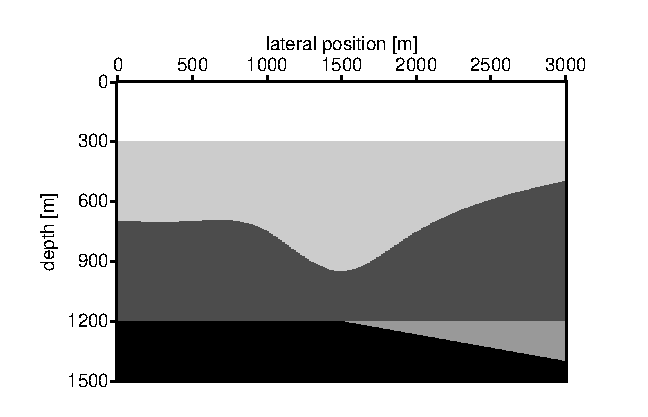
\epsfig{file=EPS/model.eps,width=12cm}}
%	\psgrid
\end{pspicture}
\caption{ Syncline model which is used in the demo directory to illustrate the working of the programs. } \label{model}
\end{figure}
%

\begin{figure}[hb]
  \begin{pspicture}(14,7)
    \put(0.0,-0.3){\epsfig{file=EPS/wave.eps}}
    \put(5.0,-0.3){\epsfig{file=EPS/wavefreq.eps}}
%	\psgrid
\end{pspicture}
\caption{ Ricker wavelet(left) and amplitude spectrum(right) which is used in the modeling experiments of the demo directoty. } \label{wave}
\end{figure}
%



\newpage
\section{\label{migr}migr / migr\_mpi}

\subsection{General}
Shot record migration scheme based on optimized x-w wave field extrapolation operators. 

There is also a parallel version of {\tt migr} called {\tt migr\_mpi}. The parallelisation is based on MPI and the number of shot gathers to be migrated is divided over the number of available working processors. For reading the shot records the master processors reads all the shots and sent the data to the working processors. If a working processor has finished its migration the image (and eventually extrapolated source and receiver wavefields) are communicated back to the master processor, who will write the data to output file(s). 

\subsection{Parameters}
Via the command-line or in a parameter file: {\tt par=$<$parameter\_file$>$}.
{\footnotesize
\begin{verbatim}
 MIGR - pre-stack depth migration (x-w).
  
 migr file_shot= file_vel= [optional parameters]
  
 Required parameters:
 
   file_shot= ............... input data to be migrated
   file_vel= ................ gridded velocity file for receiver field
   file_vels=file_vel ....... gridded velocity file for source field
  
 Optional parameters:
 
   conjg=0 .................. 1: take complex conjugate of input data
   key=sx ................... input data sorting key for receiver field
   nxmax=512 ................ maximum number of traces in input file
   ntmax=1024 ............... maximum number of samples/trace in input file
 MIGRATION 
   imc=1 .................... image condition (*)
   ndepth=all ............... number of depth steps
   zrcv=oz .................. receiver depth level
   ixa=tan(alpha)*ndepth*dz . number of traces after acquisition aperture
   ixb=ixa .................. number of traces before acquisition aperture
   ntap=0 ................... number of taper points at boundaries
   eps_a=0.0 ................ absolute stabilization factor for imc=[1,2]
   eps_r=0.001 .............. relative stabilization factor for imc=[1,2]
   domain=1 ................. 1: x-w lateral variant convolution, 0: kx-w
   zomigr=0 ................. 1: zero-offset migration (=> velocity *= 0.5)
            ................. 2: zero-offset migration (=> velocity *= 1.0)
 SOURCE DEFINITION 
   file_src=<file_name> ..... (areal)wavelet used 
   key_src=fldr ............. input data sorting key for source field
   fmin=0 ................... minimum frequency 
   fmax=70 .................. maximum frequency
   conjgs=0 ................. 1: take complex conjugate of source wavefield
   selev=0 .................. 0: ignore headers for source/receiver depth
 EXTRAPOLATION OPERATOR DEFINITION 
   select=10 ................ type of x-w operator (*)
   opl=25 ................... length of the convolution operator (odd)
   alpha=65 ................. maximum angle of interest
   perc=0.15 ................ smoothness of filter edge
   weight=5e-5 .............. weight factor in WLSQ operator calculation
   beta=3 ................... 2 < beta < 10; factor for KAISER window
   fine=10 .................. fine sampling in operator table
   filter=1 ................. apply kx-w filter to desired operator
   limit=1.0002.............. maximum amplitude in best operators
   opl_min=15 ............... minimum length of convolution operator
 OUTPUT DEFINITION 
   file_image= .............. output file with migrated result
   writeafter=10 ............ writes image/shots after # processed shots
   file_ishot=NULL .......... output file for migrated shot-records
   writeshots=0 ............. 1; writes migrated shot record
   writeinc=1 ............... trace increment of file_ishots
   verbose=0 ................ =1: shows various parameters and results
   sx_file= ................. file with extrapolated source field
   rx_file= ................. file with extrapolated receivers
   depthex= ................. depth to save extrapolated fields (m)
  
   Options for select:
         - 0 = Truncated operator
         - 1 = Gaussian tapered operator
         - 2 = Kaiser tapered operator
         - 3 = Smoothed Phase operator
         - 4 = Weighted Least Squares operator
         - 5 = Remez exchange operator
         - 8 = Smooth Weighted Least Squares operator (careful if dz<0.5*dx)
         - 9 = Optimum Smooth Weighted Least Squares operator
         - 10= Optimum Weighted Least Squares operator (Default)
   Imaging condition:
         - 0 = correlation
         - 1 = stabilized inversion
         - 2 = stabilized Least Squares
         - 4 = 2*data.r for zero-offset migration only
         - 5 = smoothed imaging P265 EAGE 2006: A. Guitton
 
  The shot and receiver positions in the model are determined by
  the hdr values gx and sx. The data from file_shot is extrapolated 
  backward, the data from file_src is extrapolated forward.
  If file_src is not set a spike is taken, if file_src=pipe read from stdin
  Note that with the conjg and conjgs options the extrapolation 
  direction can be changed.
 
  Copyright 1997, 2008 Jan Thorbecke, (janth@xs4all.nl) 

\end{verbatim}}

\subsection{General parameter description}

The shots to be migrated ({\tt file\_shot}) and the gridded subsurface files ({\tt file\_vel} and {\tt file\_vels}) should have the same lateral extend being defined by the {\tt gx} headers.  The position of the receivers of the data in the subsurface grid is done by means of the {\tt gx} header value of the velocity model corresponding to the {\tt gx} header value in the data to be extrapolated. The distance between the traces in the velocity model should be smaller or equal to the distance between the receivers/shots. The program assigns the {\tt gx} value of the receivers to the nearest grid point in the velocity model. The number of depth steps is controlled with the parameter {\tt ndepth=}. To avoid reflections at the edges of the model the parameter {\tt ntap} can be set. {\tt ntap} indicates the number of points at the edges for which a spatial taper is designed according to: $\exp{(-(0.4*(ntap-ix)/ntap)^2)}$. Choosing {\tt ntap} equal to half of the operator length is an optimimum value. 
 
Topography is taken into account by using a velocity model which has zero velocities above the defined topography. In that case the position of the source and receivers is lowered into the velocity model until a non-zero velocity is found. From that depth the extrapolation of that point is started. 

The parameter {\tt file\_src} describes the source wavelet. If {\tt file\_src} is not defined a band-limited spike is assumed. If {\tt file\_src} contains only one trace it is assumed that this trace is the wavelet used for all shots to be migrated. If {\tt file\_src} contains more than one trace it is interpreted as an areal shot record and areal short-record migration is carried out. 

The parameters {\tt ixa} and {\tt ixb} determine the number of traces to be included in the calculation of a image gather. 
{\tt ixa} defines the number of traces to include in the calculation with a lateral position greater than the lateral extend (max value of {\tt sx,gx}) of the shot gather ({\tt a} from after). 
{\tt ixb} defines the number of traces to include in the calculation with a lateral shot position smaller than the lateral extend (max value of {\tt sx,gx}) of the shot gather ({\tt b} from before).


For a more detailed discussion on the different parameters which are related to the extrapolation operator optimization the reader is referred to the description of the program \htmlref{{\bf opercalc}}{opercalc}. The WLSQ operators are described in Thorbecke et al. (2004).

\subsection{Examples}

Generating a pulse repsonse through the medium of Figure \ref{model}. 

{\footnotesize
\begin{verbatim}
migr file_shot=ricker_shift.su file_vel=syncline_cp.su zomigr=1 file_image=migr8.su verbose=1 ixa=301 select=8
suximage < migr8.su 
migr file_shot=ricker_shift.su file_vel=syncline_cp.su zomigr=1 file_image=migr10.su verbose=1 ixa=301 select=10
suximage < migr10.su 
\end{verbatim}}

%
\begin{figure}[hb]
  \begin{pspicture}(8,4.2)
    \put(-0.5,-0.3){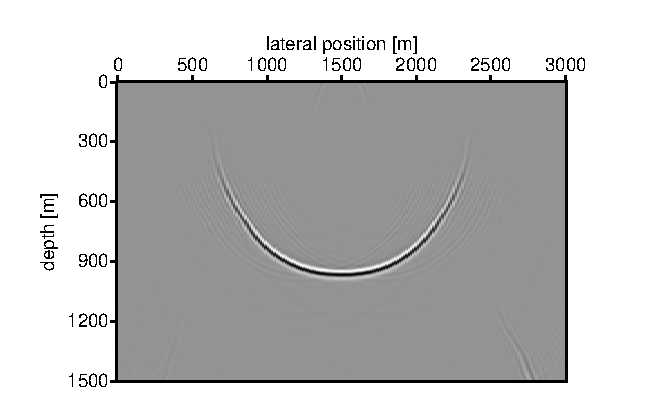
\epsfig{file=EPS/migr_puls8.eps,height=5cm}}
    \put(7.0,-0.3){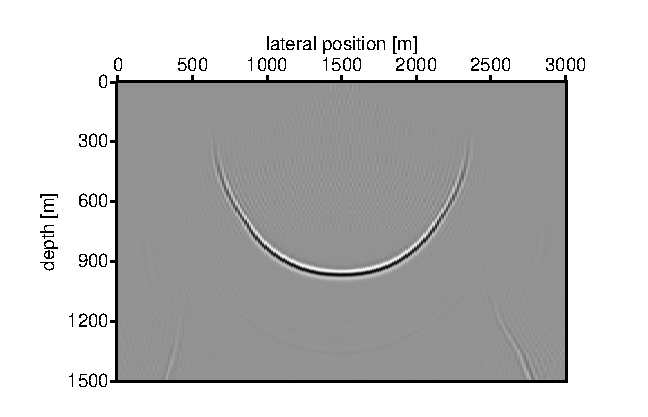
\epsfig{file=EPS/migr_puls10.eps,height=5cm}}
\end{pspicture}
\caption{ Pulse responses of the migration program for two different operators. Left show the smooth WSLQ operator and right
shows the best selected WLSQ operator.} \label{migr1}
\end{figure}
%


\subsection{To do}
3D extension is available on request.

\subsection{References}

Thorbecke, J., Wapenaar, K.,  and Swinnen, G., 2004, Design of one way wavefield extrapolation operators, using smooth functions in WLSQ optimization.: {\bf Geophysics}, pages 1037--1045.

\newpage
\section{extrap} \label{extrap}

\subsection{General}

Extrap extrapolates (forward or inverse) an input wave-field through a gridded subsurface model. The output is the extrapolated
wave-field at the desired depth, which is controlled by the parameter {\tt zrcv=}. As a special option snapshots {\tt snap=1} and/or beams {\tt beam=1} can be calculated. The snapshots option selects at every depth step the samples at the desired snapshot times. The snapshot option can be used to see how a certain wavefield propagates through a medium. The beam option gives insight how the energy of the wavefield propagates through the medium. 

For most velocity distributions the extrapolation works fine and gives good results. However for large depth steps (defined through the velocity model) and laterally very strong variations the program may give inferior result due to the assumption that within the length of the convolution operator the velocity is assumed to be homogeneous (velocity is taken at the mid-point of the operator). 

\subsection{Parameters}

Via the command-line or in a parameter file: {\tt par=$<$parameter\_file$>$}.
{\footnotesize
\begin{verbatim}
  
 extrap - forward or inverse extrapolation (x-w)
  
 extrap file_in= file_vel= file_out= [optional parameters]
  
 Required parameters:
 
   file_in= ................. Input file to be extrapolated
   file_vel= ................ gridded velocity file 
   file_out= ................ output file with extrapolated result
  
 Optional parameters:
 
   fmin=0 ................... minimum frequency 
   fmax=70 .................. maximum frequency
   mode=1 ................... type of extrapolation (1=forward, -1=inverse)
   conjg=0 .................. take complex conjugate of input data
   nxmax=512 ................ maximum number of traces in input file
   ntmax=1024 ............... maximum number of samples/trace in input file
   zstart=0 ................. depth to start extrapolation
 RECEIVER POSITIONS 
   xrcv1=ox ................. x-position of the receiver (m)
   xrcv2=ox+(nx-1)*dx ....... x-position of last receiver
   dxrcv=dx ................. step in receiver x-direction
   zrcv1=oz+(nz-1)*dz ....... z-position of the receiver (m)
   zrcv2=zrcv1 .............. z-position of last receiver
   dzrcv=0 .................. step in receiver z-direction
   xrcv= .................... x-position's of receivers (array)
   zrcv=(nz-1)*dz ........... z-position of the receivers (last depth level)
   lint=1 ................... linear interpolate between the rcv points
   file_int= ................ input file describing the interfaces (makemod)
   boundary=1 ............... boundary to place the receivers(overrules zrcv)
 EXTRAPOLATION OPERATOR DEFINITION 
   domain=0 ................. 0: x-w, 1: kx-w operator
   select=4 ................. type of x-w operator
   opl=25 ................... length of the convolution operator (odd)
   alpha=65 ................. maximum angle of interest
   perc=0.15 ................ smoothness of filter edge
   weight=5e-5 .............. weight factor in WLSQ operator calculation
   fine=10 .................. fine sampling in operator table
   filter=1 ................. apply kx-w filter to desired operator
   ntap=0 ................... number of taper points at boundaries
   limit=1.0002.............. maximum amplitude in best operators
   opl_min=15 ............... minimum length of convolution operator
 SNAPSHOTS DEFINITION (if snap=1) 
   tsnap1=-nt*dt/2........... first snapshot time (s)
   tsnap2=nt*dt/2 ........... last snapshot time (s)
   dtsnap=25*dt ............. snapshot time interval (s)
   reverse=0 ................ extrapolate from deepest level back to surface
 OUTPUT 
   snap=0 ................... snapshots
   beam=0 ................... beams
   verbose=0 ................ silent option; >0 display info
 
   Options for select:
         - 0 = Truncated operator
         - 1 = Gaussian tapered operator
         - 2 = Kaiser tapered operator
         - 3 = Smoothed Phase operator
         - 4 = Weighted Least Squares operator
         - 5 = Remez exchange operator
         - 8 = Smooth Weighted Least Squares operator
         - 9 = Optimum Smooth Weighted Least Squares operator
         - 10= Optimum Weighted Least Squares operator
 
  Copyright 1997, 2008 Jan Thorbecke, (janth@xs4all.nl) 

\end{verbatim}}

\subsection{General parameter description}

The data to be extrapolated ({\tt file\_in}) and the gridded subsurface ({\tt file\_vel}) should at least have the same number of
traces. If the number of traces of the subsurface is smaller an error message is the result. If the number of traces is bigger then
the user should position the first receiver of the data in the subsurface grid. This is done by setting the {\tt gx} header value of
the velocty model corresponding to the {\tt gx} header value in the data to be extrapolated. The distance between the traces in both
gathers should be equal. The number of depth steps is controlled with the parameter {\tt zrcv=} and the extrapolation direction is controlled with {\tt mode=}. For inverse extrapolation the complex conjugate of the forward extrapolation operator is taken. The parameter {\tt reverse} extrapolated the data from the deepest level in the velocity model to the lowest level. 

Topography is taken into account by using a velocity model which has zero velocities above the defined topography. In that case the position of the source and receivers is lowered into the velocity model until a non-zero velocity is found. From that depth the extrapolation of that point is started. 

To avoid reflections at the edges of the model the parameter {\tt ntap} can be set. {\tt ntap} indicates the number of points at the edges for which a spatial taper is designed according to: $\exp{(-(0.4*(ntap-ix)/ntap)^2)}$. Choosing {\tt ntap} equal to half of the operator length is an optimimum value.

The parameter {\tt snap=1} gives at the defined snapshot times (with {\tt tsnap1, tsnap2} and {\tt dtsnap}) the extrapolated wave-field. With this option the propagation of the wavefield through the model can be monitored. 

The parameter {\tt beam=1} gives the energy of the extrapolated wave-field at all calculated depth steps. The energy is calculated in the frequency domain for all depth steps according to $E(x,d) = {1 \over nfreq} \sum_{\omega} \|data(x, \omega)\|^{1 \over 2}$. With this option the propagation of the energy through the model can be monitored. 

The receiver spread is defined by coordinates in x ({\tt xrcv, dxrcv}) and z ({\tt zrcv dzrcv}). The parameters {\tt xrcv} and {\tt zrcv} are defined as arrays which interpretation depends on the parameter {\tt lint}. For example if {\tt xrcv=0,3000}, {\tt zrcv=0,0}, {\tt dxrcv=15}, {\tt dzrcv=0} and {\tt lint=1} then between the points (0,0) and (3000,0) the defined receiver positions are calculated by a linear interpolation between the two points with dx=15, which results in an receiver array of 201 receivers ranging from (0,0) to (3000,0). However, if {\tt lint=0} the receivers are only defined at the points (0,0) and (3000,0). One can also use the paremeters {\tt xrcv1, xrcv2} and {\tt zrcv1, zrcv2} to define receiver arrays.

For a more detailed discussion on the different parameters which are related to the extrapolation operator optimization the reader is referred to the description of the program \htmlref{{\bf opercalc}}{opercalc}. The WLSQ operators are described in Thorbecke et al. (2004).

\subsection{Examples}

In the following example a Green's function in a medium is calculated which gives the data we want to extrapolate. By choosing in
{\bf extrap} the options {\tt beam=1} and {\tt conjg=1}, the calculated output shows how the energy is focused to depth position
1000 (the source depth of the input file) and gets defocused again for deeper depth positions. The options {\tt snap=1} and {\tt
conjg=1} show snapshots of the wavefield propagating through the model.  

{\footnotesize
\begin{verbatim}

cfpmod file_vel=syncline_cp.su xsrc1=1500 zsrc1=1200 ntap=30 file_src=ricker.su file_out=green.su

extrap file_in=green.su file_vel=syncline_cp.su verbose=1 beam=1 conjg=1 | suximage 

extrap file_in=green.su file_vel=syncline_cp.su verbose=1 snap=1 conjg=1 \
	tsnap1=-0.512 dtsnap=0.128 | suximage 

\end{verbatim}}

%
\begin{figure}[hb]
  \begin{pspicture}(8,4.2)
    \put(-0.5,-0.3){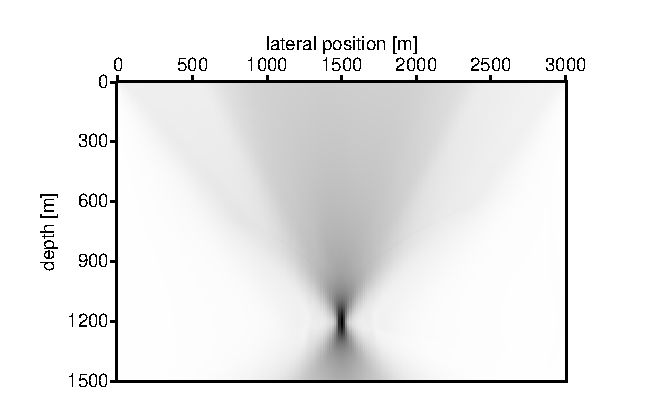
\epsfig{file=EPS/extrap_beam.eps,height=5cm}}
    \put(7.0,-0.3){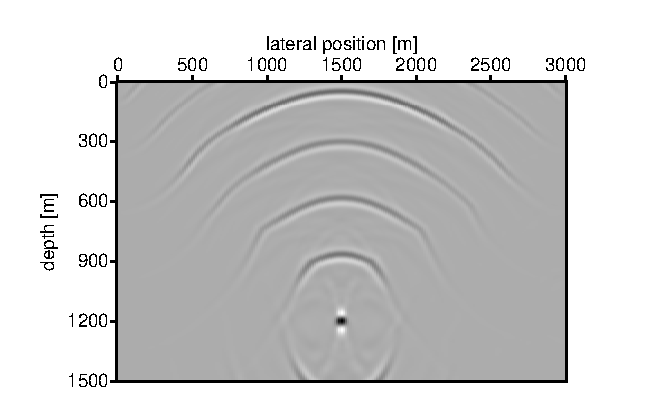
\epsfig{file=EPS/extrap_snap.eps,height=5cm}}
\end{pspicture}
\caption{Inverse extrapolated results of Green's function placed in the middle of the model of Figure \ref{model} at z=1200 m. The
left picture shows the energy beam of the extrapolated wavefield and the right picture show snapshots of the converging wavefield. } \label{extrap1}
\end{figure}
%

For forward extrapolation of the data through the model the following command can be given (to let the extrapolation stop at a certain depth level use the parameter {\tt zrcv=}):

{\footnotesize
\begin{verbatim}
extrap file_in=green.su file_vel=syncline_cp.su verbose=1 mode=-1 zrcv=1200 | suximage 
\end{verbatim}}

Now with cfpmod from surface to depth and then with extrap from depth back to surface:

{\footnotesize
\begin{verbatim}

cfpmod file_vel=syncline_cp.su xsrc1=1500 zsrc1=0 zrcv=1200 ntap=30 file_src=ricker.su file_out=deep.su

extrap file_in=deep.su file_vel=syncline_cp.su verbose=1 zrcv=0 zstart=1200 reverse=1 mode=-1 verbose=1 | suximage 

\end{verbatim}}

%
\begin{figure}[hb]
  \begin{pspicture}(8,5.2)
    \put(-0.5,-0.3){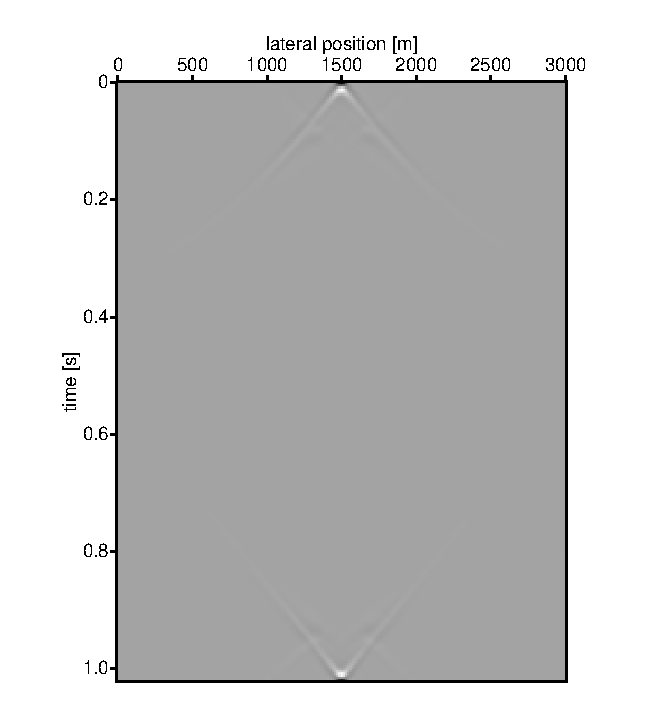
\epsfig{file=EPS/extrap_z1200.eps,height=6cm}}
    \put(7.0,-0.3){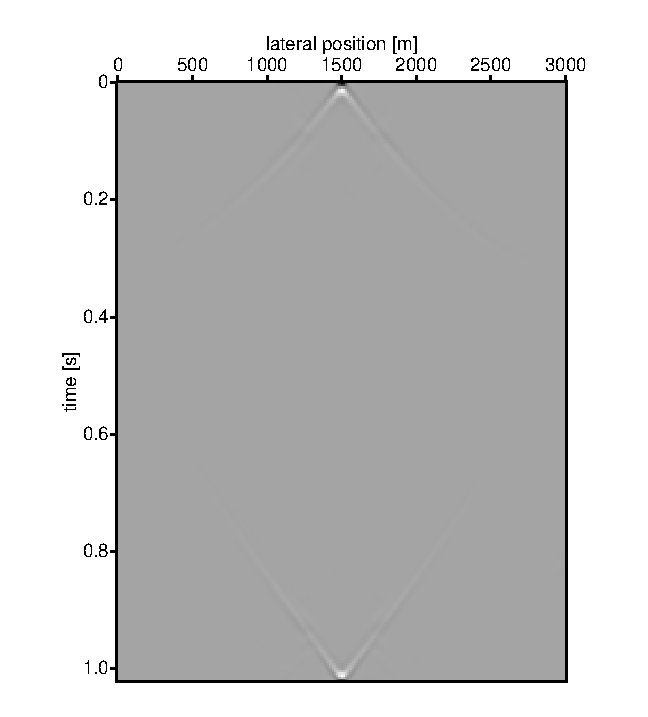
\epsfig{file=EPS/extrap_z0.eps,height=6cm}}
\end{pspicture}
\caption{Inverse extrapolated wavefields of Green's function placed in the middle of the model of Figure \ref{model} at z=1200 m.
(left) the right picture show the result of a source at the surface and receivers at z=1200 m.} \label{extrap2}
\end{figure}
%
\subsection{To do}
Extension of the operator optimization algorithms to 3D media, this extension is already available in a non-official release version and can be obtained on request.

\subsection{References}

Thorbecke, J., Wapenaar, K.,  and Swinnen, G., 2004, Design of one way wavefield extrapolation operators, using smooth functions in WLSQ optimization.: {\bf Geophysics}, pages 1037--1045.


\newpage
\section{\label{cfpmod}cfpmod}

\subsection{General}

Based on the same algorithm as used in the program {\bf extrap}, {\bf cfpmod} calculates pulse responses of sources which are defined in the subsurface. This program is therefore very usefull for the generation of CFP operators. 
\subsection{Parameters}

Via the command-line or in a parameter file: {\tt par=$<$parameter\_file$>$}.

{\footnotesize
\begin{verbatim}
  
 cfpmod - modeling one-way travel times in x-w domain
 
 cfpmod file_vel= xsrc1= zsrc1= [optional parameters]
  
 Required parameters:
 
   file_vel= ................ gridded velocity file
   xsrc1= ................... x-position of the source (m)
   zsrc1= ................... z-position of the source (m)
  
 Optional parameters:
  
   file_out= ................ output file with traveltimes
   file_int= ................ input file describing the interfaces (makemod)
   mode=1 ................... type of extrapolation (1=forward, -1=inverse)
   ntap=0 ................... number of taper points at boundaries
   n2max=512 ................ maximum number of traces in input file
   n1max=1024 ............... maximum number of samples/trace in input file
 SOURCE POSITIONS 
   xsrc2=xsrc1 .............. x-position of last source
   dxsrc=0 .................. step in source x-direction
   zsrc2=zsrc1 .............. z-position of last source
   dzsrc=0 .................. step in source z-direction
   boundary=0 ............... boundary to place the sources (overrules zsrc)
 RECEIVER POSITIONS 
   xrcv1=ox ................. x-position of the receiver (m)
   xrcv2=ox+(nx-1)*dx ....... x-position of last receiver
   dxrcv=dx ................. step in receiver x-direction
   zrcv1=oz ................. z-position of the receiver (m)
   zrcv2=zrcv1 .............. z-position of last receiver
   dzrcv=0 .................. step in receiver z-direction
   xrcv= .................... x-position's of receivers (array)
   dxspr=0 .................. step of receiver spread in x-direction
   zrcv=0 ................... z-position of the receivers (first depth level)
   lint=1 ................... linear interpolate between the rcv points
 SAMPLING AND SOURCE DEFINITION 
   file_src=<file_name> ..... wavelet in time used (overrules dt)
   file_amp=<file_name> ..... wavelet in lateral direction 
   wnx=1 .................... number of lateral wavelet samples
   dt=0.004 ................. stepsize in time-direction 
   nt=256 ................... number of time samples
   fmin=0 ................... minimum frequency 
   fmax=70 .................. maximum frequency
   add=0 .................... 1: adds all defined sources
 PLANE WAVE AREAL SHOT RECORD DEFINITION (only calculated if Na != 0)
   amin=-65 ................. minimum angle of plane wave illumination
   amax=-amin ............... maximum angle of plane wave illumination
   Na=0 ..................... number of plane waves between amin and amax
 Note that the plane waves cannot be added together by using add=1 
 EXTRAPOLATION OPERATOR DEFINITION 
   select=4 ................. type of x-w operator
   opl=25 ................... length of the convolution operator (odd)
   alpha=65 ................. maximum angle of interest
   perc=0.15 ................ smoothness of filter edge
   weight=5e-5 .............. weight factor in WLSQ operator calculation
   fine=10 .................. fine sampling in operator table
   filter=1 ................. apply kx-w filter to desired operator
   limit=1.0002.............. maximum amplitude in best operators
   opl_min=15 ............... minimum length of convolution operator
 OUTPUT 
   beam=0 ................... 1 beams, 2 add all beams for all defined shots
   verbose=0 ................ silent option; >0 display info
  
   Options for select:
         - 0 = Truncated operator
         - 1 = Gaussian tapered operator
         - 2 = Kaiser tapered operator
         - 3 = Smoothed Phase operator
         - 4 = Weighted Least Squares operator
         - 5 = Remez exchange operator
         - 8 = Smooth Weighted Least Squares operator
         - 9 = Optimum Smooth Weighted Least Squares operator
         - 10= Optimum Weighted Least Squares operator
  
  Copyright 1997, 2008 Jan Thorbecke, (janth@xs4all.nl) 
\end{verbatim}}

\subsection{General parameter description}

The gridded subsurface ({\tt file\_vel}) which is needed in the caclulation can be made with for example the DELPHI program {\bf makemod}. {\tt file\_int} is defined by the same program. 

The source position(s) are defined by coordinates in x({\tt xsrc1, xsrc2, dxsrc}) and z ({\tt zsrc1, zsrc2, dzsrc}). If {\tt file\_int} is defined then it is also possible to use the parameter {\tt boundary} instead of the z parameters. The interface file ({\tt file\_int}) is used to place the source at the defined boundary (at the defined x position). Every source postition defines one output gather. However if {\tt add=1} the defined source postions are combined to a planar source and only one output gather is calculated.

The receiver spread is defined by coordinates in x ({\tt xrcv, dxrcv}) and z ({\tt zrcv dzrcv}). The parameters {\tt xrcv} and {\tt zrcv} are defined as arrays which interpretation depends on the parameter {\tt lint}. For example if {\tt xrcv=0,3000}, {\tt zrcv=0,0}, {\tt dxrcv=15}, {\tt dzrcv=0} and {\tt lint=1} then between the points (0,0) and (3000,0) the defined receiver positions are calculated by a linear interpolation between the two points with dx=15, which results in an receiver array of 201 receivers ranging from (0,0) to (3000,0). However, if {\tt lint=0} the receivers are only defined at the points (0,0) and (3000,0). One can also use the paremeters {\tt xrcv1, xrcv2} and {\tt zrcv1, zrcv2} to define receiver arrays.
 
Once the spread for the first shot position is defined, the parameter {\tt dxspr} define the movement of the spread for the next shot.  Choosing {\tt dxspr=0} defines a fixed spread modeling.

The parameter {\tt file\_src} defines a source wavelet, however, if this parameter is not defined a wavelet with a flat spectrum and zero phase is used in the program. 
The sources can be extended in the lateral direction by using the parameter {\tt wnx} or {\tt file\_amp}.  If there are more source positions defined (with {\tt zsrc1 $\not=$ zsrc2} and {\tt dzsrc > 0}) the output consists of a number of shot gathers. The source position in the gridded model is chosen at the nearest grid position.

Plane waves are defined by using the parameters {\tt Na}, {\tt amin} and {\tt amax}. Which define the number of plane waves and the minimum and maximum angle respectively. 

For a more detailed discussion on the different parameters which are related to the operator optimization the reader is referred to the description of the program \htmlref{{\bf opercalc}}{opercalc}.

\subsection{Examples}

To run the program a gridded velocity file has to be defined. We use the gridded velocity file (synclin\_cp.su, see Figure
\ref{model}) which can
be found in the demo directory, and a ricker wavelet (ricker.su, see Figure \ref{wave}), which can also be found in the demo directory.

In this gridded subsurface file we want to place a source at depth 1000 m, at x-position 500 and model the response at the surface.
The result is shown in Figure \ref{cfp1} and the command to generate this results is:

{\footnotesize
\begin{verbatim}
../bin/cfpmod file_vel=syncline_cp.su xsrc1=1000 zsrc1=500 ntap=30 file_src=ricker.su | suximage
\end{verbatim}}
%
\begin{figure}[hb]
  \begin{pspicture}(8,6.5)
    \put(5.0,-0.3){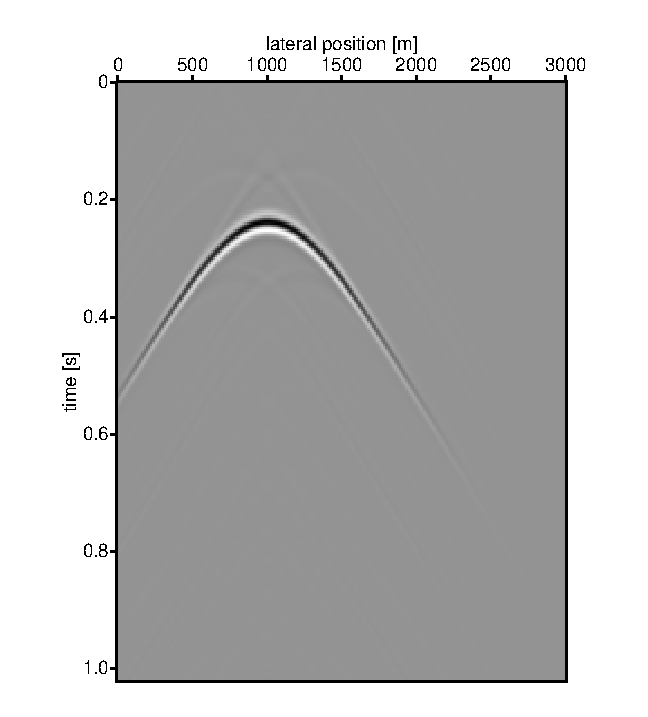
\epsfig{file=EPS/cfpmod_x1000_z500.eps,height=7cm}}
\end{pspicture}
\caption{Response of a point source at x=1000 and z=500 m., measured at the surface z=0.  } \label{cfp1}
\end{figure}
%

To calculate 5 plane wave responses, with 5 different angles ranging from -20 to 20,  from the subsurface the following command can be used:

{\footnotesize
\begin{verbatim}
../bin/cfpmod file_vel=syncline_cp.su xsrc1=1000 zsrc1=1200 ntap=30  \
    file_src=ricker.su Na=5 amin=-20 verbose=1 | suximage
\end{verbatim}}
%
\begin{figure}[hb]
  \begin{pspicture}(8,7)
    \put(-0.55,-0.3){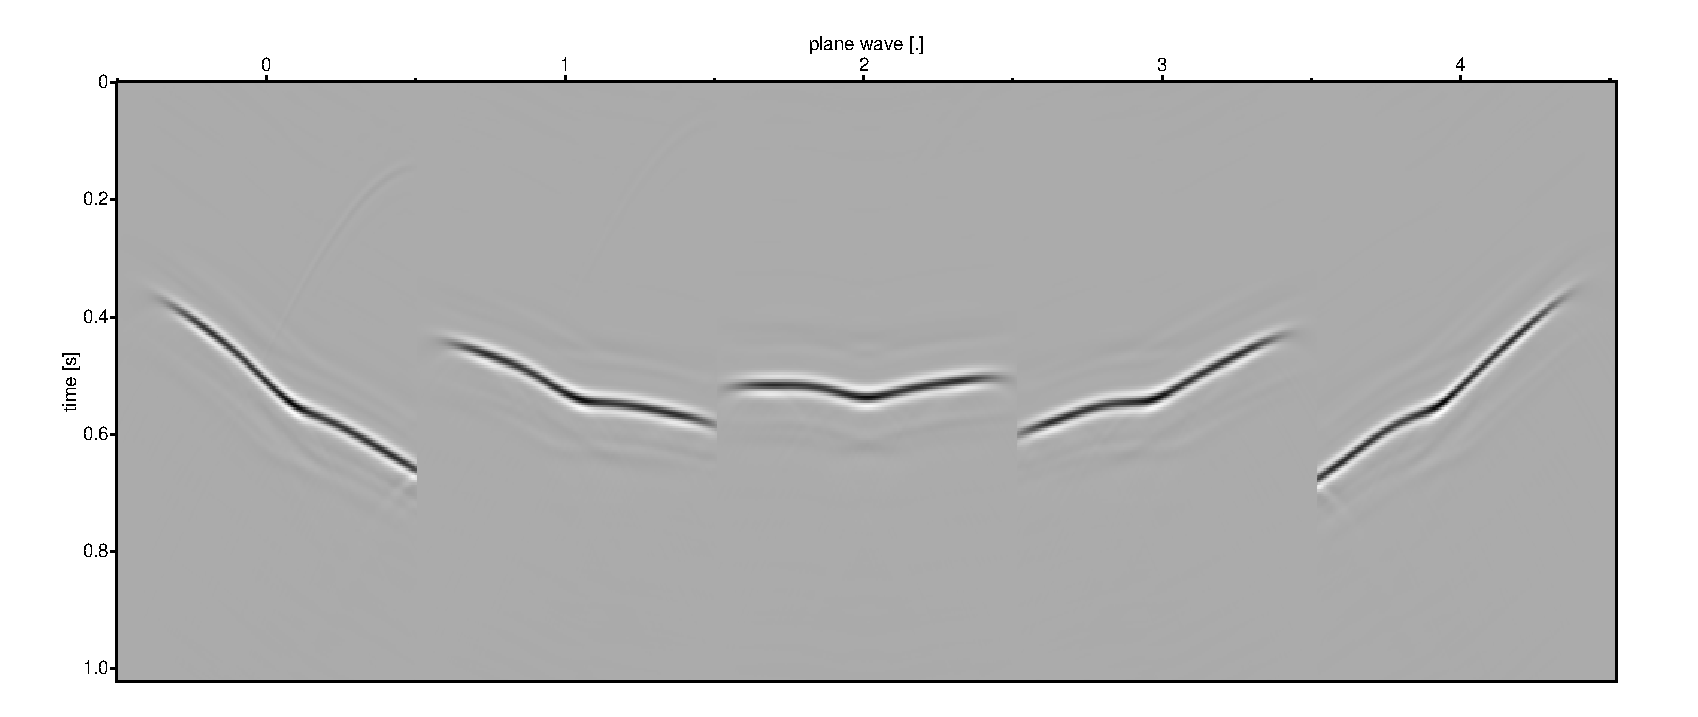
\epsfig{file=EPS/cfpmod_plane.eps,height=7cm}}
\end{pspicture}
\caption{Response of 5 plane waves at z=1200 and x=1500 with angles ranging from -20 to 20. } \label{cfp2}
\end{figure}

To model more than one source position use:

{\footnotesize
\begin{verbatim}
../bin/cfpmod file_vel=syncline_cp.su xsrc1=300 xsrc2=2700 \
    zsrc1=1200 zsrc2=1200 dxsrc=300 file_src=ricker.su \
    ntap=30 verbose=1 | suximage
\end{verbatim}}

and add those together (and do only one modeling step) do

{\footnotesize
\begin{verbatim}
../bin/cfpmod file_vel=syncline_cp.su xsrc1=300 xsrc2=2700 \
    zsrc1=1200 zsrc2=1200 dxsrc=300 file_src=ricker.su \
    ntap=30 add=1 verbose=1 | suximage
\end{verbatim}}
%
\begin{figure}[hb]
  \begin{pspicture}(8,6.5)
    \put(5.0,-0.3){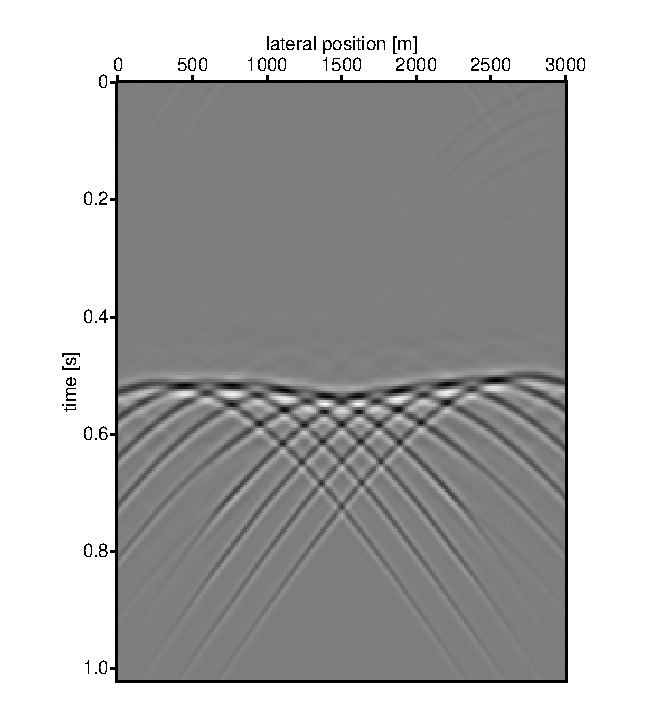
\epsfig{file=EPS/cfpmod_add.eps,height=7cm}}
\end{pspicture}
\caption{Response of several point sources position at x=[300,2700] and z=1200 m., measured at the surface z=0.  } \label{cfp3}
\end{figure}
%

\subsection{To do}
Using the local reflectivity function (or a source distribution) instead of a pulse.

Better source position definition if the source does not lie on a point defined by the subsurface grid (which is an implementation of a local extrapolation).


\newpage
\section{onewvsp} \label{onewvsp}

\subsection{General}

{\bf onewvsp} is based on the same algorithm as used in \htmlref{{\bf extrap}}{extrap}. {\bf onewvsp} can be used to generate pseudo VSP
data from seismic surface data. For the extrapolation of the data
one-way extrapolation operators (these operators can be calculated
with \htmlref{{\bf opercalc}}{opercalc}) are used.

\subsection{Parameters}

Via the command-line or in a parameter file: {\tt par=$<$parameter\_file$>$}.
{\footnotesize
\begin{verbatim}
 onewvsp - One-way VSP generation
 
 onewvsp file_in= file_vel= [optional parameters]
 
 Required parameters:
 
   file_in= ................. Input file
   file_vel= ................ gridded velocity file 
 
 Optional parameters:
 
   file_vsp= ................ Output file of calculated VSP
   file_ex= ................. Output file with the extrapolated result
   file_over= ............... writes model file with vsp positions
   nxmax=512 ................ maximum number of traces in input file
   ntmax=1024 ............... maximum number of samples/trace in input file
   file_init= ............... filename for ProMax IO initialization
   line=1  .................. 1: black lines; 0: white lines in overlay
   verbose=0 ................ silent option; >0 display info
 RECEIVER POSITIONS 
   xrcv=0 ................... x-position's of receivers (array)
   zrcv=0,nz*dz ............. z-position of the receivers (array)
   dxrcv=dx ................. step in receiver x-direction
   dzrcv=dz ................. step in receiver z-direction
   lint=1 ................... linear interpolate between the rcv points
   dxspr=0 .................. step of receiver spread in x-direction
   nvsp=1 ................... number of VSP positions
 EXTRAPOLATION 
   mode=-1 .................. type of extrapolation (1=forward, -1=inverse)
   fmin=0 ................... minimum frequency
   fmax=70 .................. maximum frequency
   ntap=0 ................... number of taper points at boundaries
 EXTRAPOLATION OPERATOR DEFINITION 
   select=4 ................. type of x-w operator
   opl=25 ................... length of the convolution operator (odd)
   alpha=65 ................. maximum angle of interest
   perc=0.15 ................ smoothness of filter edge
   weight=5e-5 .............. weight factor in WLSQ operator calculation
   fine=10 .................. fine sampling in operator table
   filter=1 ................. apply kx-w filter to desired operator
   limit=1.0002.............. maximum amplitude in best operators
   opl_min=15 ............... minimum length of convolution operator
  
   Options for select:
         - 0 = Truncated operator
         - 1 = Gaussian tapered operator
         - 2 = Kaiser tapered operator
         - 3 = Smoothed Phase operator
         - 4 = Weighted Least Squares operator
         - 5 = Remez exchange operator
         - 8 = Smooth Weighted Least Squares operator
         - 9 = Optimum Smooth Weighted Least Squares operator
         - 10= Optimum Weighted Least Squares operator
 
   The weighting factor is used in the convolution operator calculation.
   This calculation is done in an optimized way.
   The default weight factor is for most cases correct. For a more stable
   operator chooce a weight factor closer to 1, if 1 is chosen no 
   optimization is carried out and the convolution operator is the 
   truncated Inverse Fourier Transform of the Kx-w operator.
   The non-optimized operator is the truncated IFFT of a smooth Kx-w 
   operator. This operator is designed by Gerrit Blacquiere.
 
   Note that all coordinates are related to the velocity model.
 
  Copyright 1997, 2008 Jan Thorbecke, (janth@xs4all.nl) 
 
      initial version   : 14-12-1993 (j.w.thorbecke@tudelft.nl)
          version 1.0   : 11-10-1995 (release version)
          version 2.0   : 23-06-2008 (janth@xs4all.nl) 2008
\end{verbatim}}

\noindent

\subsection{General parameter description}

The input files are the same as for the program \htmlref{{\bf
    extrap}}{extrap}. The data to be extrapolated ({\tt file\_in}) and
the gridded subsurface ({\tt file\_vel}) should at least have the same
number of traces. If the number of traces of the subsurface is smaller
an error message is the result. If the number of traces is bigger then
the user should position the first receiver of the data in the
subsurface grid. In no correct hdrs ({\tt gx} and {\tt sx}) are
available this can be done with the parameter {\tt rpos}, which
indicates the tracenumber (an integer) in the subsurface grid where
the first receiver is positioned. The distance between the traces in
both gathers should be equal. The extrapolation direction is
controlled with {\tt mode=}. For inverse extrapolation the complex
conjugate of the forward extrapolation operator is taken.

To avoid reflections at the edges of the model the parameter {\tt
  ntap} can be set. {\tt ntap} indicates the number of points at the
edges for which a spatial taper is designed according to:
$\exp{(-(0.4*(ntap-ix)/ntap)^2)}$. Choosing {\tt ntap} equal to half
of the operator length is an optimimum value.

The output file {\tt file\_vsp} contains the pseudo VSP records for
the different VSP positions. If {\tt file\_over} is defined the VSP
positions are overlayed on the gridded velocity model. Displaying the
{\tt file\_over} file gives an overview of the chosen VSP positions.
{\tt file\_ex} (if defined) contains the extrapolated data which is
extrapolated upto the deepest receiver in the VSP array.

The receiver positions of the VSP array are defined with the
parameters {\tt xrcv}, {\tt zrcv}, {\tt dxrcv}, {\tt dzrcv}, and {\tt
  lint}. If {\tt xrcv} and {\tt zrcv} are not defined the default
receiver array is calculated. This receiver array is positioned at x=0
for all depth positions in the gridded subsurface model. If {\tt xrcv}
is defined with only one value (e.g. {\tt xrcv=1500}) then the VSP is
positioned at x=xrcv for all defined depth positions. Note that {\tt
  dzrcv} defines at which depth postions receivers should be placed.
Choosing an array for {\tt zrcv} (e.g. {\tt zrcv=0,2000}) gives only
positions inbetween the defined depth array. For a deviated VSP
configuration both {\tt xrcv} and {\tt zrcv} should be defined as
arrays (e.g. {\tt xrcv=1000,1000,1500 zrcv=0,2000,3000}). The
parameter {\tt lint} set to 1 calculates (with {\tt dxrcv} and {\tt
  dzrcv} defined) inbetween the given positions the receiver array
(use the {\tt file\_over} option to see how the receivers are
positioned). If {\tt lint} is set to 0 then only the receiver postions
at every pair of {\tt xrcv} and {\tt zrcv} are chosen (in the previous
example only three postions).

The parameters {\tt nvsp} and {\tt dxspr} give the posibility to
define more than one receiver arrays, {\tt nvsp} defines the number of
arrays and {\tt dxspr} gives the distance between the receiver arrays.
The first receiver array is defined with {\tt xrcv}, {\tt zrcv}, {\tt
  dxrcv}, {\tt dzrcv}, and {\tt lint} (see above). The other receiver
arrays have the same structure but are calculated at x-positions which
are dxspr moved (use the \\ {\tt file\_over} option to see how the
receivers are positioned).

For a more detailed discussion on the different parameters which are
related to the operator optimization the reader is referred to the
description of the program \htmlref{{\bf opercalc}}{opercalc}.

\subsection{Examples}

{\footnotesize
\begin{verbatim}onewvsp file_vel= file_vsp= file_over= 
\end{verbatim}}

\subsection{To do}
Nothing really.


\newpage
\section{opercalc} \label{opercalc}

\subsection{General}
The program {\bf opercalc} calculates extrapolation operators for a given frequency. This program uses the same algorithm as is used in the programs \htmlref{{\bf extrap}}{extrap}, \htmlref{{\bf cfpmod}}{cfpmod} and \htmlref{{\bf migr}}{migr}. This program can be used to check whether the defined parameters for the calculation of the operator table are correct. It also showes how the different optimization algortihms distort the spatial-frequency spectrum of the extrapolation operator.

\subsection{Parameters}

Via the command-line or in a parameter file: {\tt par=$<$parameter\_file$>$}.
{\footnotesize
\begin{verbatim}
 opercalc - calculates extrapolation operators for a given frequency
 
 opercalc  file_out= [optional parameters] > Kx-file and X-file
 
 Required parameters:
 
   file_out= ................ base name of the output file(s)
 
 Optional parameters:
 
   freq=20 .................. frequency at which the operator is calculated
   c=2000 ................... velocity of the medium
   dx=15 .................... stepsize in spatial direction
   dz=dx .................... extrapolation step
   nkx=512 .................. number of kx samples
 EXTRAPOLATION OPERATOR DEFINITION 
   opl=25 ................... length of the convolution operator (odd)
   alpha=65 ................. maximum angle of interest
   perc=0.15 ................ smoothness of filter edge
   amp=0.5 .................. amplitude smooth operator
   weight=5e-5 .............. weight factor in WLSQ operator calculation
   filter=1 ................. using filter in kx-w domain before WLSQ
   beta=3 ................... 2 < beta < 10; factor for KAISER window
   nbw=3 .......... ......... order of butterworth filter
 OUTPUT DEFINITION 
   cycle=0 .................. 1; units along kx-axis set to 1.0/nkx
   on_su_pipe=0 ............. 1: x or 2: Kx results on SU-pipe
   verbose=0 ................ >0: shows various parameters and results
 
 The two files produced have a _x or _kx extension in the filename.
 The _x-file contains the optimized convolution operators (9x). 
 The _kx-file contains the spatial spectrum of the operators (10x):
         - 1 = Truncated operator
         - 2 = Gaussian tapered operator
         - 3 = Kaiser tapered operator
         - 4 = Smoothed Phase operator
         - 5 = Weighted Least Squares operator
         - 6 = Remez exchange operator
         - 7 = Hankel function H_1(2)
         - 8 = Non-linear CFSQP optimization
         - 9 = Smooth WLSQ operator
         - 10= Exact operator (phase shift)
 
  Copyright 1997, 2008 Jan Thorbecke, (janth@xs4all.nl) 
 
     intitial version   : 14-12-1993 (j.w.thorbecke@tudelft.nl)
          version 1.0   : 17-10-1995 (release version)
          version 2.0   : 23-06-2008 (janth@xs4all.nl) 2008
\end{verbatim}}
\noindent
{\bf NOTE:} This program can be run using the same parameter setup or parameter file as the other main programs of the EXTRAP directory.

\subsection{File formats}

The two files produced have a \_x or \_kx extension in the filename.
The x-file contains the optimized operators (7 traces) in the spatial domain.
The kx-file has 9 traces with trace number:

\hangindent=1.cm \hangafter=0
(1) Truncated operator \\ (2) Gaussian tapered operator \\ (3) Kaiser tapered operator \\  (4) Smoothed Phase operator \\ (5) Weighted least-squares \\ (6) Remez exchange operator \\ (7) Hankel function H$_1$(2) \\ (8) Non-linear CFSQP optimization \\ (9) smooth WLSQ operator \\ (10) Exact operator 

\subsection{General parameter description}

All are set to default values. The operators are computed in the wavenumber domain for all wavenumber values defined. The operators
are transformed back to the spatial domain, with or without an optimization step. The optimization is described  in Thorbecke (2004). Parameter {\tt nkx} defines the number of operator points in the wavenumber domain (double sided number). Parameter {\tt opl} defines the number of operator points in the space domain (double sided number, odd). Parameters {\tt dx} and and {\tt dz} define the spatial sampling intervals, parameter {\tt c} the velocity, {\tt freq} the frequency. The parameter {\tt alpha} defines the minimum and maximum angle of the extrapolation operators. The optimization using least-squares is controlled via the parameters {\tt weight}, {\tt alpha} and {\tt perc}.

The parameter {\tt alpha} defines the wavenumber window for which the optimization is carried out. The influence of the wavenumbers outside this window is taken to be less important. The importance of the wavenumbers outside the window is described by the parameter {\tt weight}. If {\tt weight=1} then all wavenumbers are equally important for the optimization and the 'optimized' result is in fact a truncation. For weighting values less than one the wavenumbers outside the wavenumber band of interest are less important. A very small weight factor can give rise to unstable results so in order to remain stable in the recursion a weight factor between 1.e-4 and 1e-7 is most convenient. The parameter {\tt perc} describes over which bandwidth the wavenumber spectrum is filtered. It is defined as the fraction of the band of interest over which the filtering is carried out.

The output is arranged via the parameters {\tt file\_out}, {\tt on\_su\_pipe} and {\tt cycle}.

\subsection{Examples}

To display the default operators just type:

{\footnotesize
\begin{verbatim}
opercalc on_su_pipe=2 file_out=nep.su | suamp | suxgraph style=normal
\end{verbatim}}

for the spectra of the convolution operators, to display the spatial convolution operators type:

{\footnotesize
\begin{verbatim}
opercalc on_su_pipe=1 file_out=nep.su | suamp | suxgraph style=normal
\end{verbatim}}

%
\begin{figure}[hb]
  \begin{pspicture}(8,5.2)
    \put(-0.5,-0.3){\epsfig{file=EPS/opercalc_x.eps,height=6cm}}
    \put(7.0,-0.3){\epsfig{file=EPS/opercalc_kx.eps,height=6cm}}
\end{pspicture}
\caption{Wavefield extrapolation operators calculated by opercalc. Left shows the amplitude of the optimised operator in the spatial
domain and right shows the amplitude in the wavenumber domain. } \label{opercalc1}
\end{figure}


\subsection{To do}
Nothing really...



\end{document}
